\documentclass{article}
\usepackage{booktabs}   
\usepackage{geometry}
\usepackage{graphicx}
\usepackage{eurosym}
\usepackage{hyperref}
\geometry{margin=1in}

\title{ECB Paper Extension Financial Hubs and Home Bias in the EU}

\begin{document}
\maketitle


\section{Equity Home Bias and Euro Area Financial Integration}

Our analysis of the EWN data revealed two striking patterns. First, Euro Area 
countries exhibited a markedly stronger decline in equity home bias than 
non-Euro Area OECD countries over the sample period (Figure~\ref{fig:ewn_ehb}). 
This is consistent with the hypothesis that the introduction of the common 
currency facilitated financial integration among member states, reducing 
barriers to cross-border equity investment within the currency union. Second, 
and more puzzling, the Euro Area as a consolidated entity also exhibited a pronounced EHB decline approaching 0, 
and thus substantially exceeding that of comparable non-EA developed economies.

\begin{figure}[htbp]
    \centering
    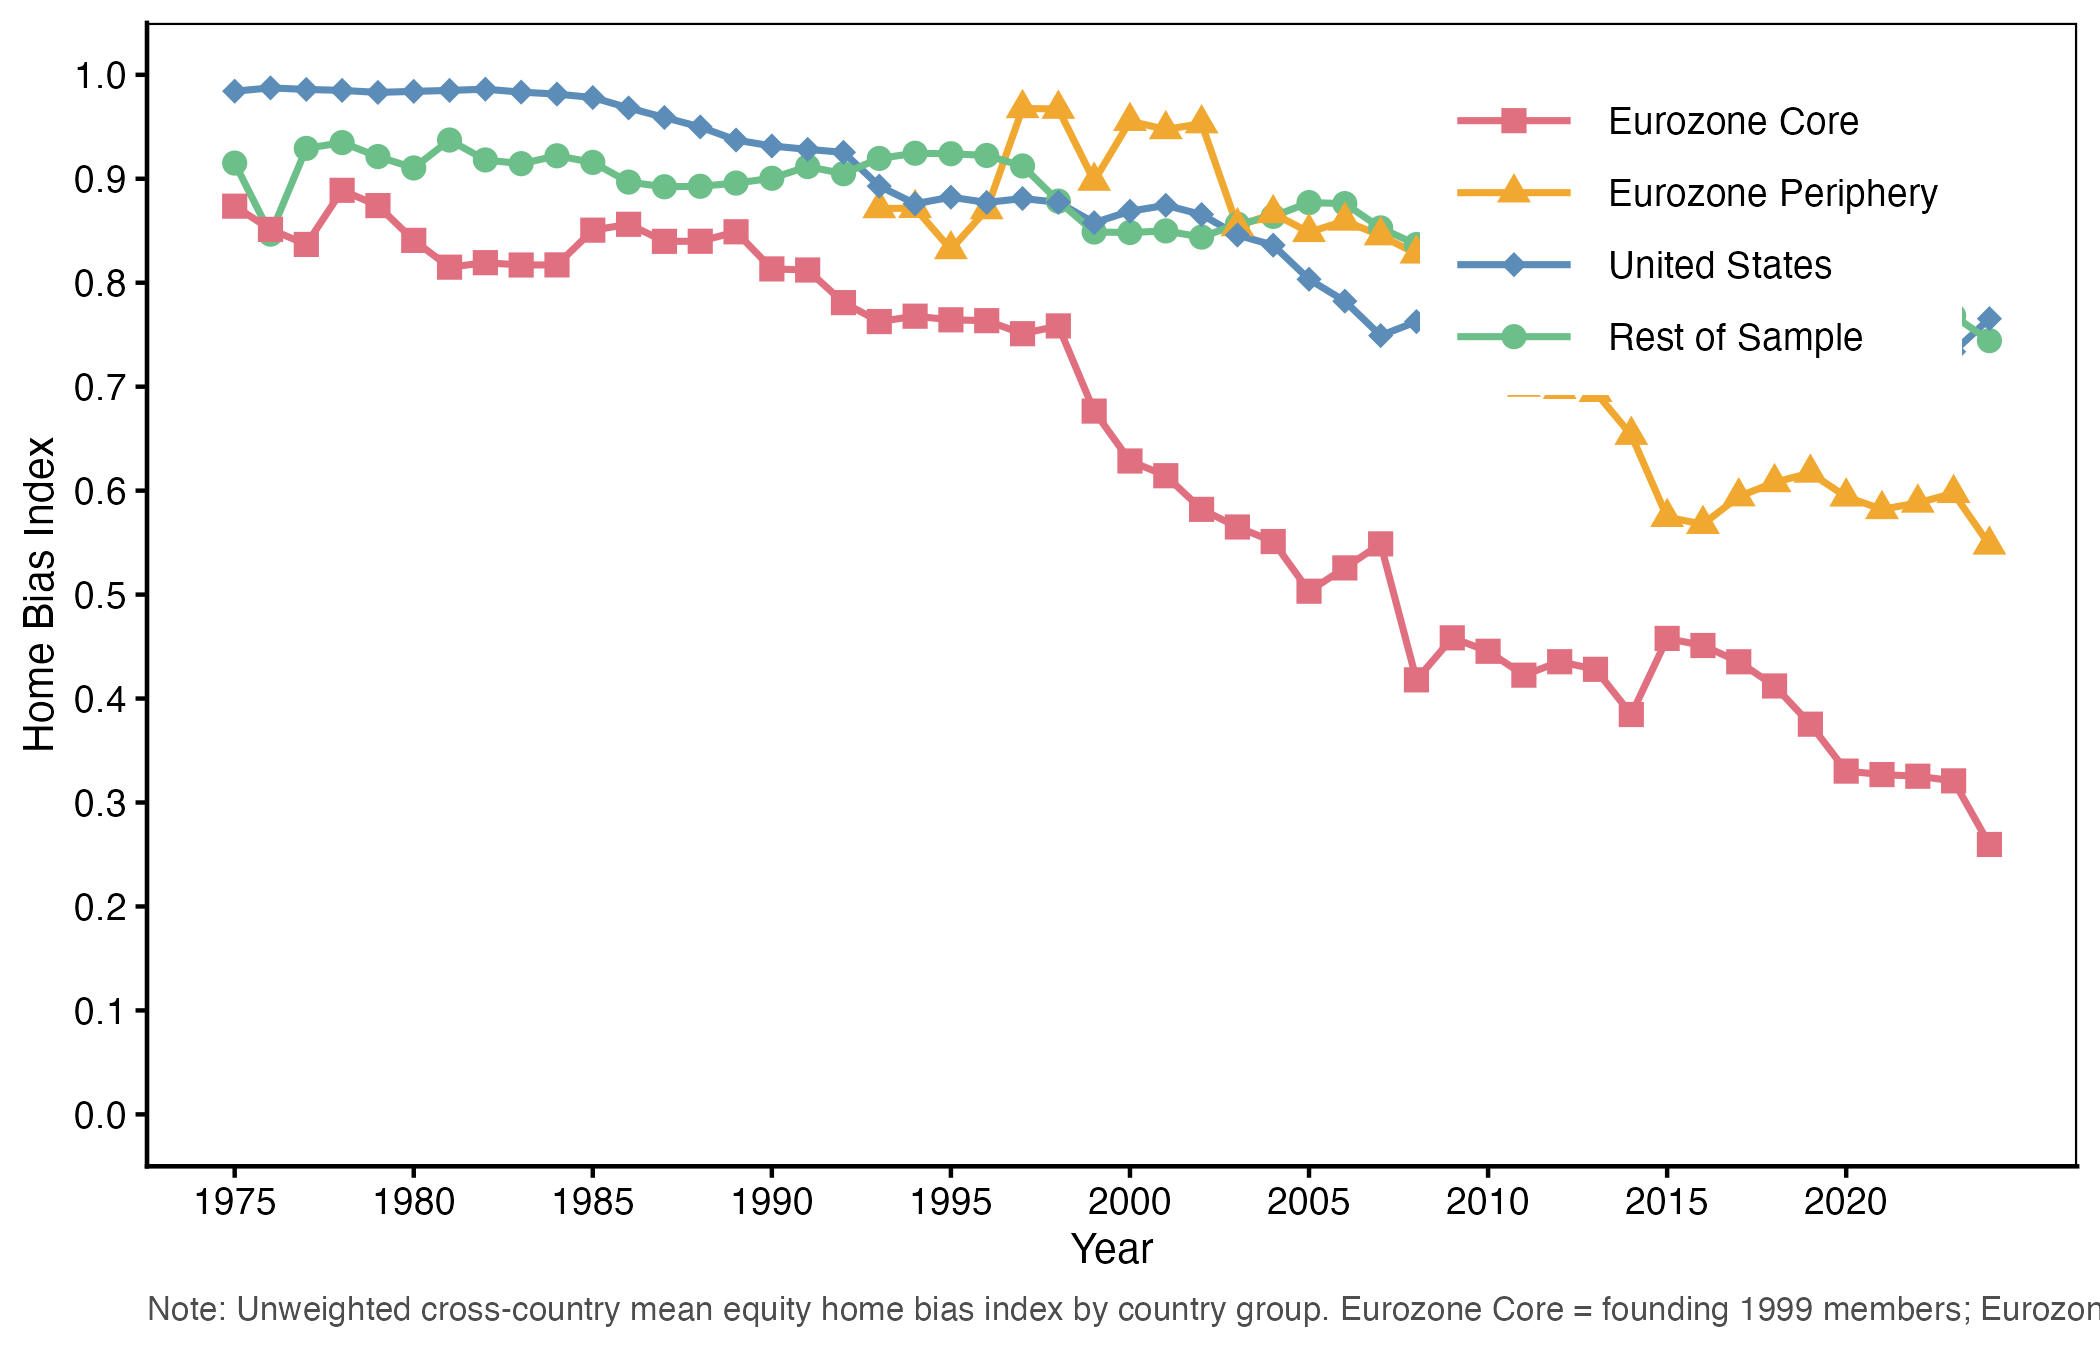
\includegraphics[width=0.9\textwidth]{../output/ehb_mean_extended_1975_2024_4groups.png}
    \caption{Equity home bias by country group, 1975--2024.}
    \label{fig:ehb_groups}
\end{figure}

\begin{figure}[htbp]
    \centering
    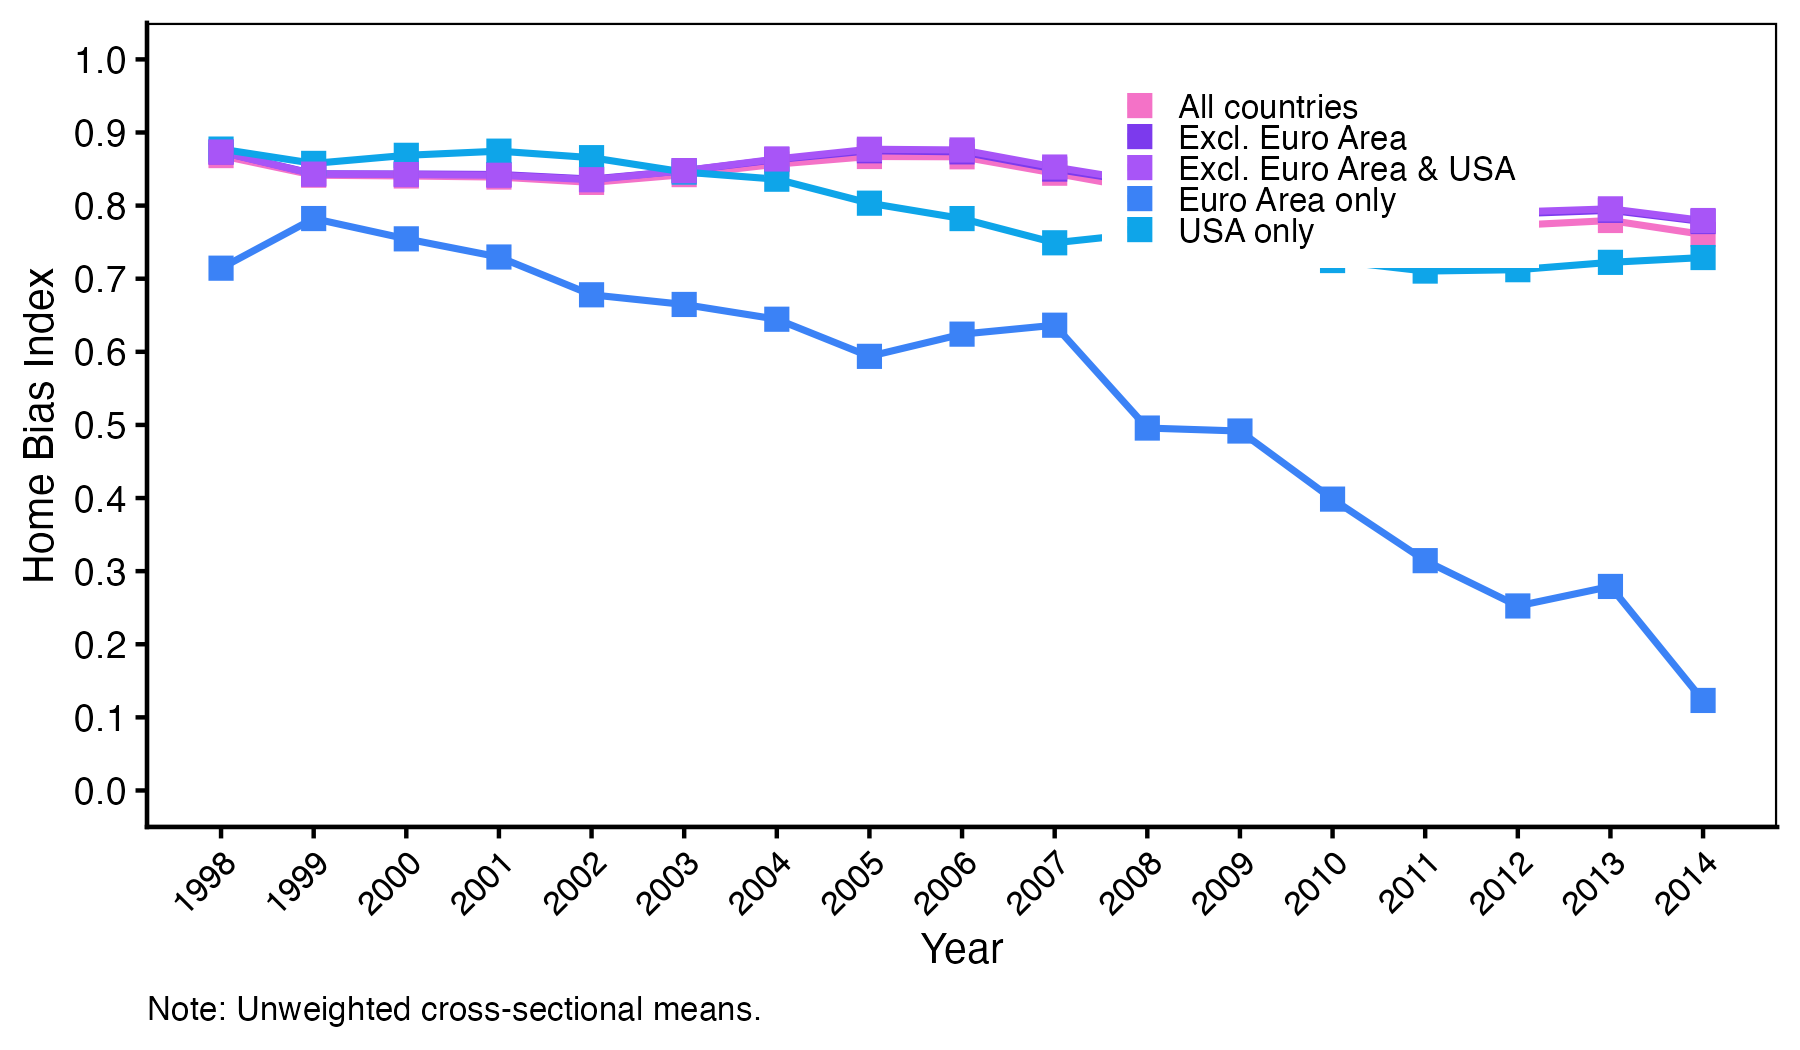
\includegraphics[width=0.9\textwidth]{../output/equity_home_bias_five_series.png}
    \caption{Equity home bias for the Euro Area aggregate, USA and rest of sample.}
    \label{fig:ehb_ea_aggregate}
\end{figure}

The second finding is difficult to reconcile based on what we would expect from Europen Integration. 
If the decline in individual countries' home bias were primarily driven by increased holdings of other Euro 
Area countries' equities (intra-EA integration), then consolidating the Euro 
Area into a single entity should reclassify these cross-border intra-EA 
positions as domestic, leaving the aggregate EHB largely unchanged relative 
to other developed economies. The fact that the aggregate declined sharply 
suggests either that EA countries also diversified substantially into 
non-EA equities, or that the underlying data suffers from measurement 
problems that inflate measured foreign equity positions.

\subsection{Measurement Distortions in Euro Area Portfolio Data}

A recent contribution by \cite{beck2024} provides a resolution to this puzzle. 
The authors demonstrate that standard international portfolio statistics---the 
International Investment Position (IIP) and the IMF's Coordinated Portfolio 
Investment Survey (CPIS)---systematically overstate the foreign equity 
positions of Euro Area countries due to the role played by what they term 
``onshore offshore financial centers'' (OOFCs): Luxembourg, Ireland, and 
to a lesser extent the Netherlands. These countries serve two functions 
that distort measured bilateral positions.

\paragraph{Fund intermediation.} Luxembourg and Ireland host large 
investment fund industries. These funds are domiciled there for regulatory 
and tax reasons (the UCITS passport, favorable withholding tax treaties), 
but their investors reside worldwide. Under standard residency-based 
accounting, when a German pension fund purchases shares in a 
Luxembourg-domiciled equity fund, this is recorded as Germany holding a 
foreign equity claim on Luxembourg---regardless of what the fund actually 
invests in. The underlying exposures (to US, Japanese, or even German 
equities) are invisible in the data. This creates two problems. First, it 
misattributes the geographic destination of investment: a claim that 
economically represents exposure to the US equity market appears as 
exposure to Luxembourg. Second, and more consequentially, a substantial 
share of the assets managed by Luxembourg and Ireland funds is owned by 
non-EA investors---the United Kingdom, United States, Switzerland, Japan, 
and others. These positions are attributed to the Euro Area in standard 
statistics because the fund is domiciled within the EA, even though the 
ultimate investors are not European.

\paragraph{Securities issuance by foreign affiliates.} Multinational 
corporations routinely establish financing subsidiaries in the Netherlands, 
Ireland, or Luxembourg for tax and regulatory purposes. When an Italian 
investor purchases a bond issued by such a subsidiary, the position is 
recorded as a claim on the subsidiary's country of residence rather than 
the parent company's home country. This channel is addressed by a 
nationality-based restatement of securities, which we do not pursue further 
here but which \cite{beck2024} document in detail.

\paragraph{Three portfolio components.} The key conceptual contribution 
of \cite{beck2024} is to decompose measured Euro Area portfolios into 
three components. The first comprises direct holdings of securities by 
EA investors---the undistorted portion of the data. The second consists 
of indirect holdings by EA investors through OOFC-domiciled funds: when 
these funds are ``unwound,'' the fund share claim on Luxembourg or Ireland 
is replaced by the underlying securities the fund actually holds. The third, 
and most problematic, component consists of positions held by 
rest-of-world investors through OOFC funds. These are spuriously 
attributed to the Euro Area under residency-based accounting.

The authors estimate that of approximately \euro 7 trillion in equities 
and bonds held by Luxembourg and Ireland funds, only around \euro 2.4 
trillion can be attributed to EA investors. The remaining \euro 4.7 
trillion belongs to the rest of the world but inflates measured EA 
positions in standard statistics. For equity home bias specifically, 
\cite{beck2024} show that after correcting for these distortions, the 
apparent excess decline in EA equity home bias relative to other developed 
economies largely disappears (their Figure 9). The corrected EA average 
EHB follows a trajectory comparable to that of the United States and 
other non-EA developed economies.

\subsection{Who Owns Luxembourg and Ireland Funds?}

To illustrate the magnitude of the attribution problem, we use the fund 
counterparty statistics compiled by \cite{beck2024} from regulatory data 
reported by the Luxembourg Commission de Surveillance du Secteur Financier 
(CSSF) and the Central Bank of Ireland. These data record the immediate 
counterparty---the investor who directly holds fund shares---by country 
or region of residence.

Figure~\ref{fig:lux_ownership} shows the composition of ownership of 
Luxembourg-domiciled fund shares from 1998 to 2021. Throughout the entire 
period, Euro Area investors (Luxembourg residents and the rest of the EA 
combined) account for less than half of total fund assets. The remaining 
share is held by investors from Switzerland, the United Kingdom, the 
United States, Japan, and other non-EA countries. In standard portfolio 
statistics, the entirety of these funds' asset holdings is attributed to 
the Euro Area. The figure also reveals that total assets under management 
grew from approximately \euro 460 billion in 1998 to over \euro 5 trillion 
by 2021 (Figure~\ref{fig:lux_ownership_levels}), implying that the 
magnitude of the misattribution has increased substantially over time---
precisely the period during which Euro Area equity home bias appeared to 
decline most rapidly.

\begin{figure}[htbp]
    \centering
    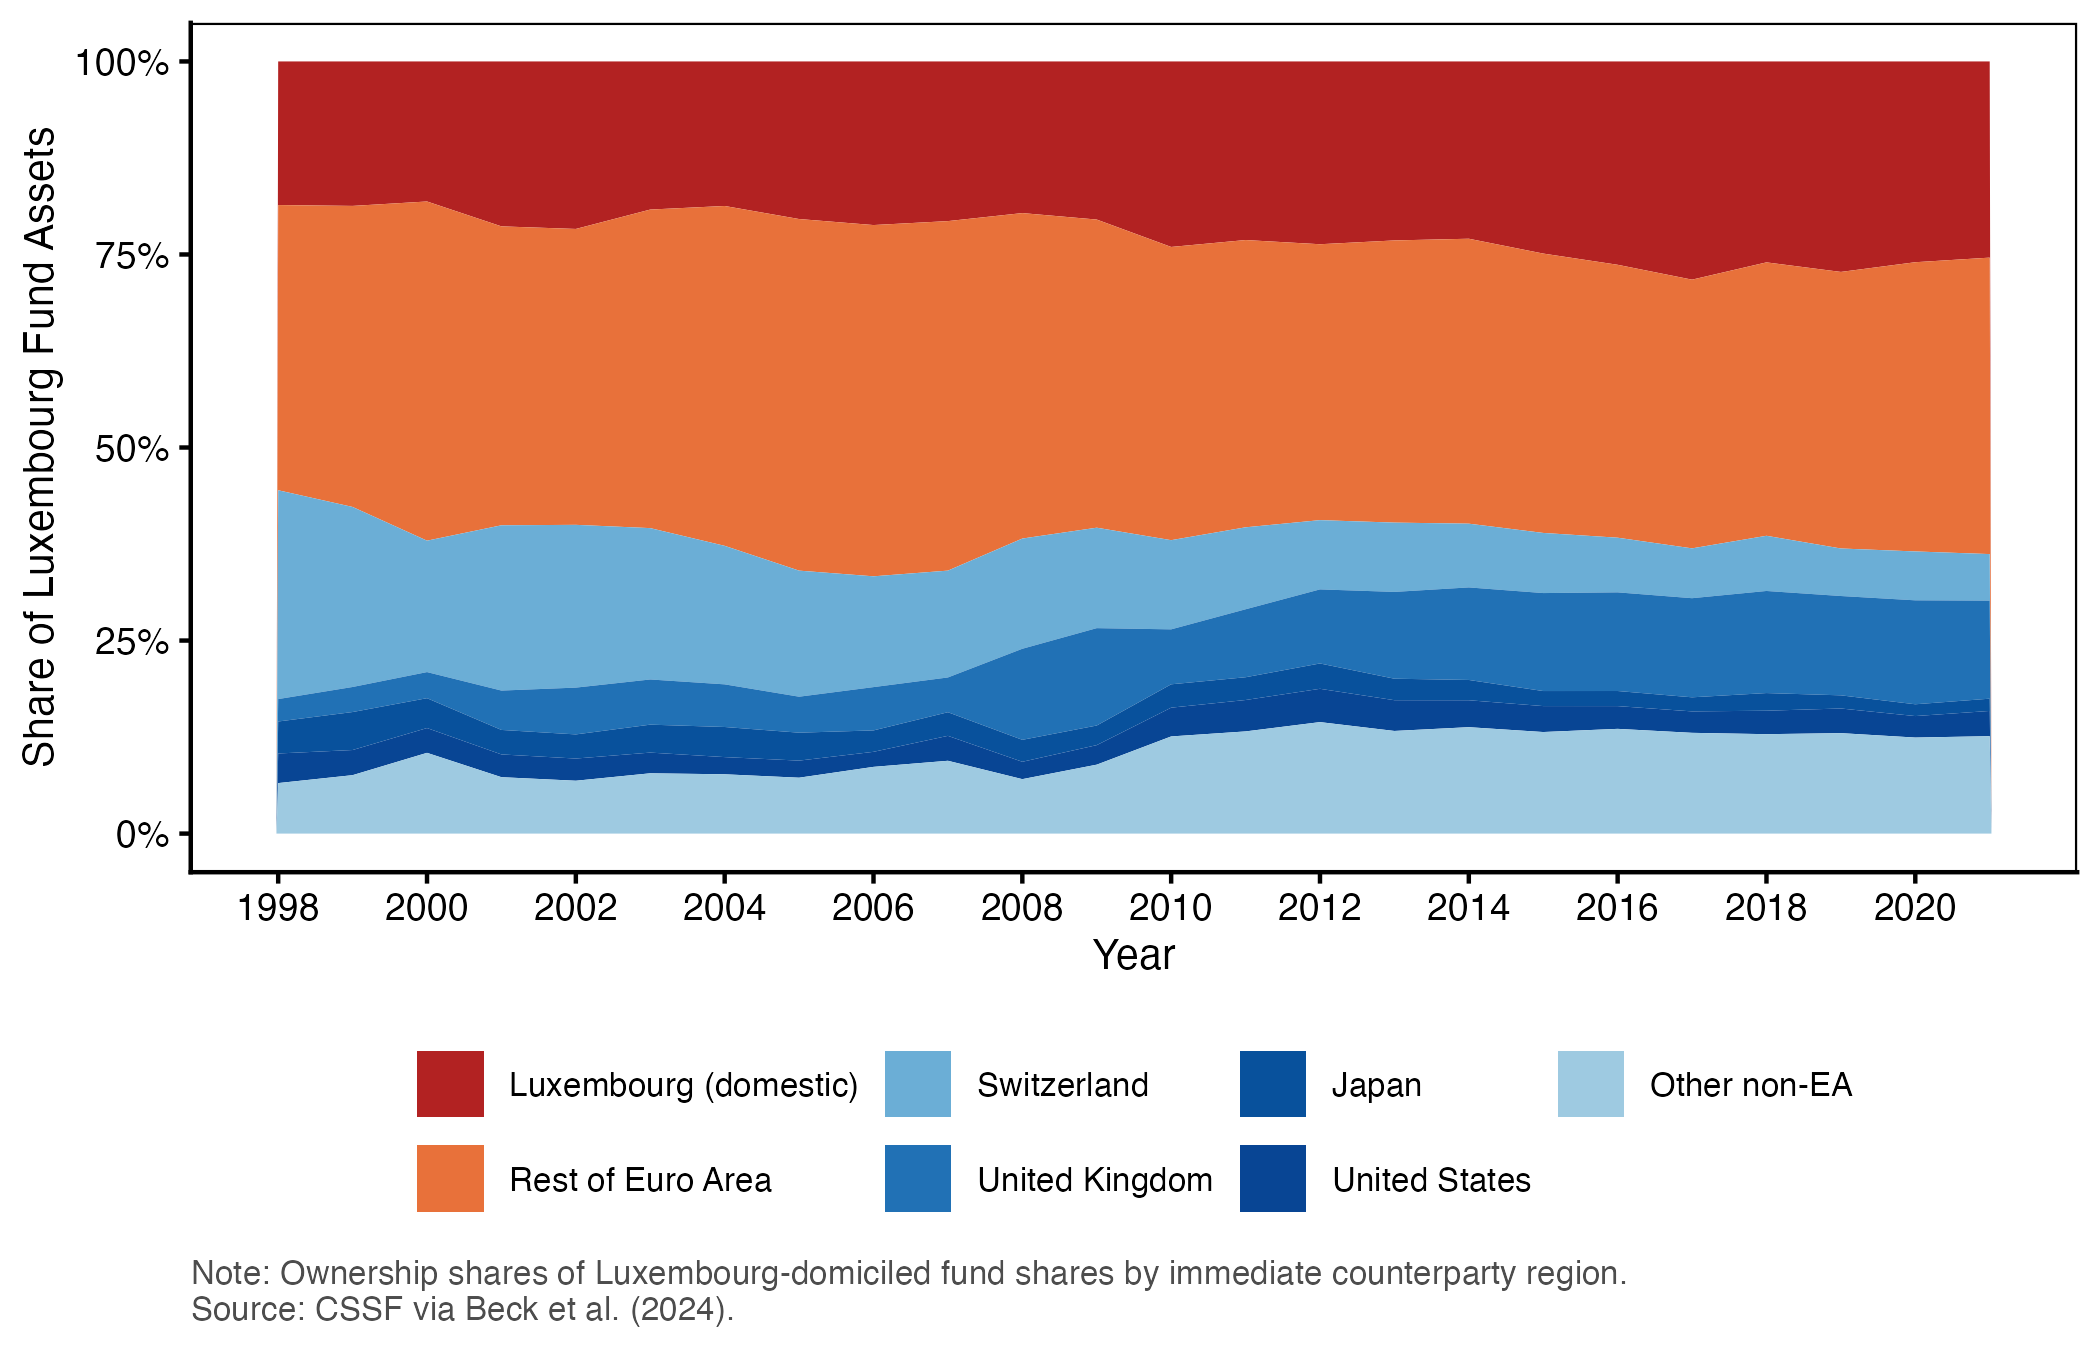
\includegraphics[width=0.9\textwidth]{../output/lux_fund_ownership_shares.png}
    \caption{Ownership composition of Luxembourg-domiciled fund shares by 
    immediate counterparty region, 1998--2021. Euro Area investors (domestic 
    Luxembourg and rest of EA) consistently account for less than half of 
    total assets.}
    \label{fig:lux_ownership}
\end{figure}

\begin{figure}[htbp]
    \centering
    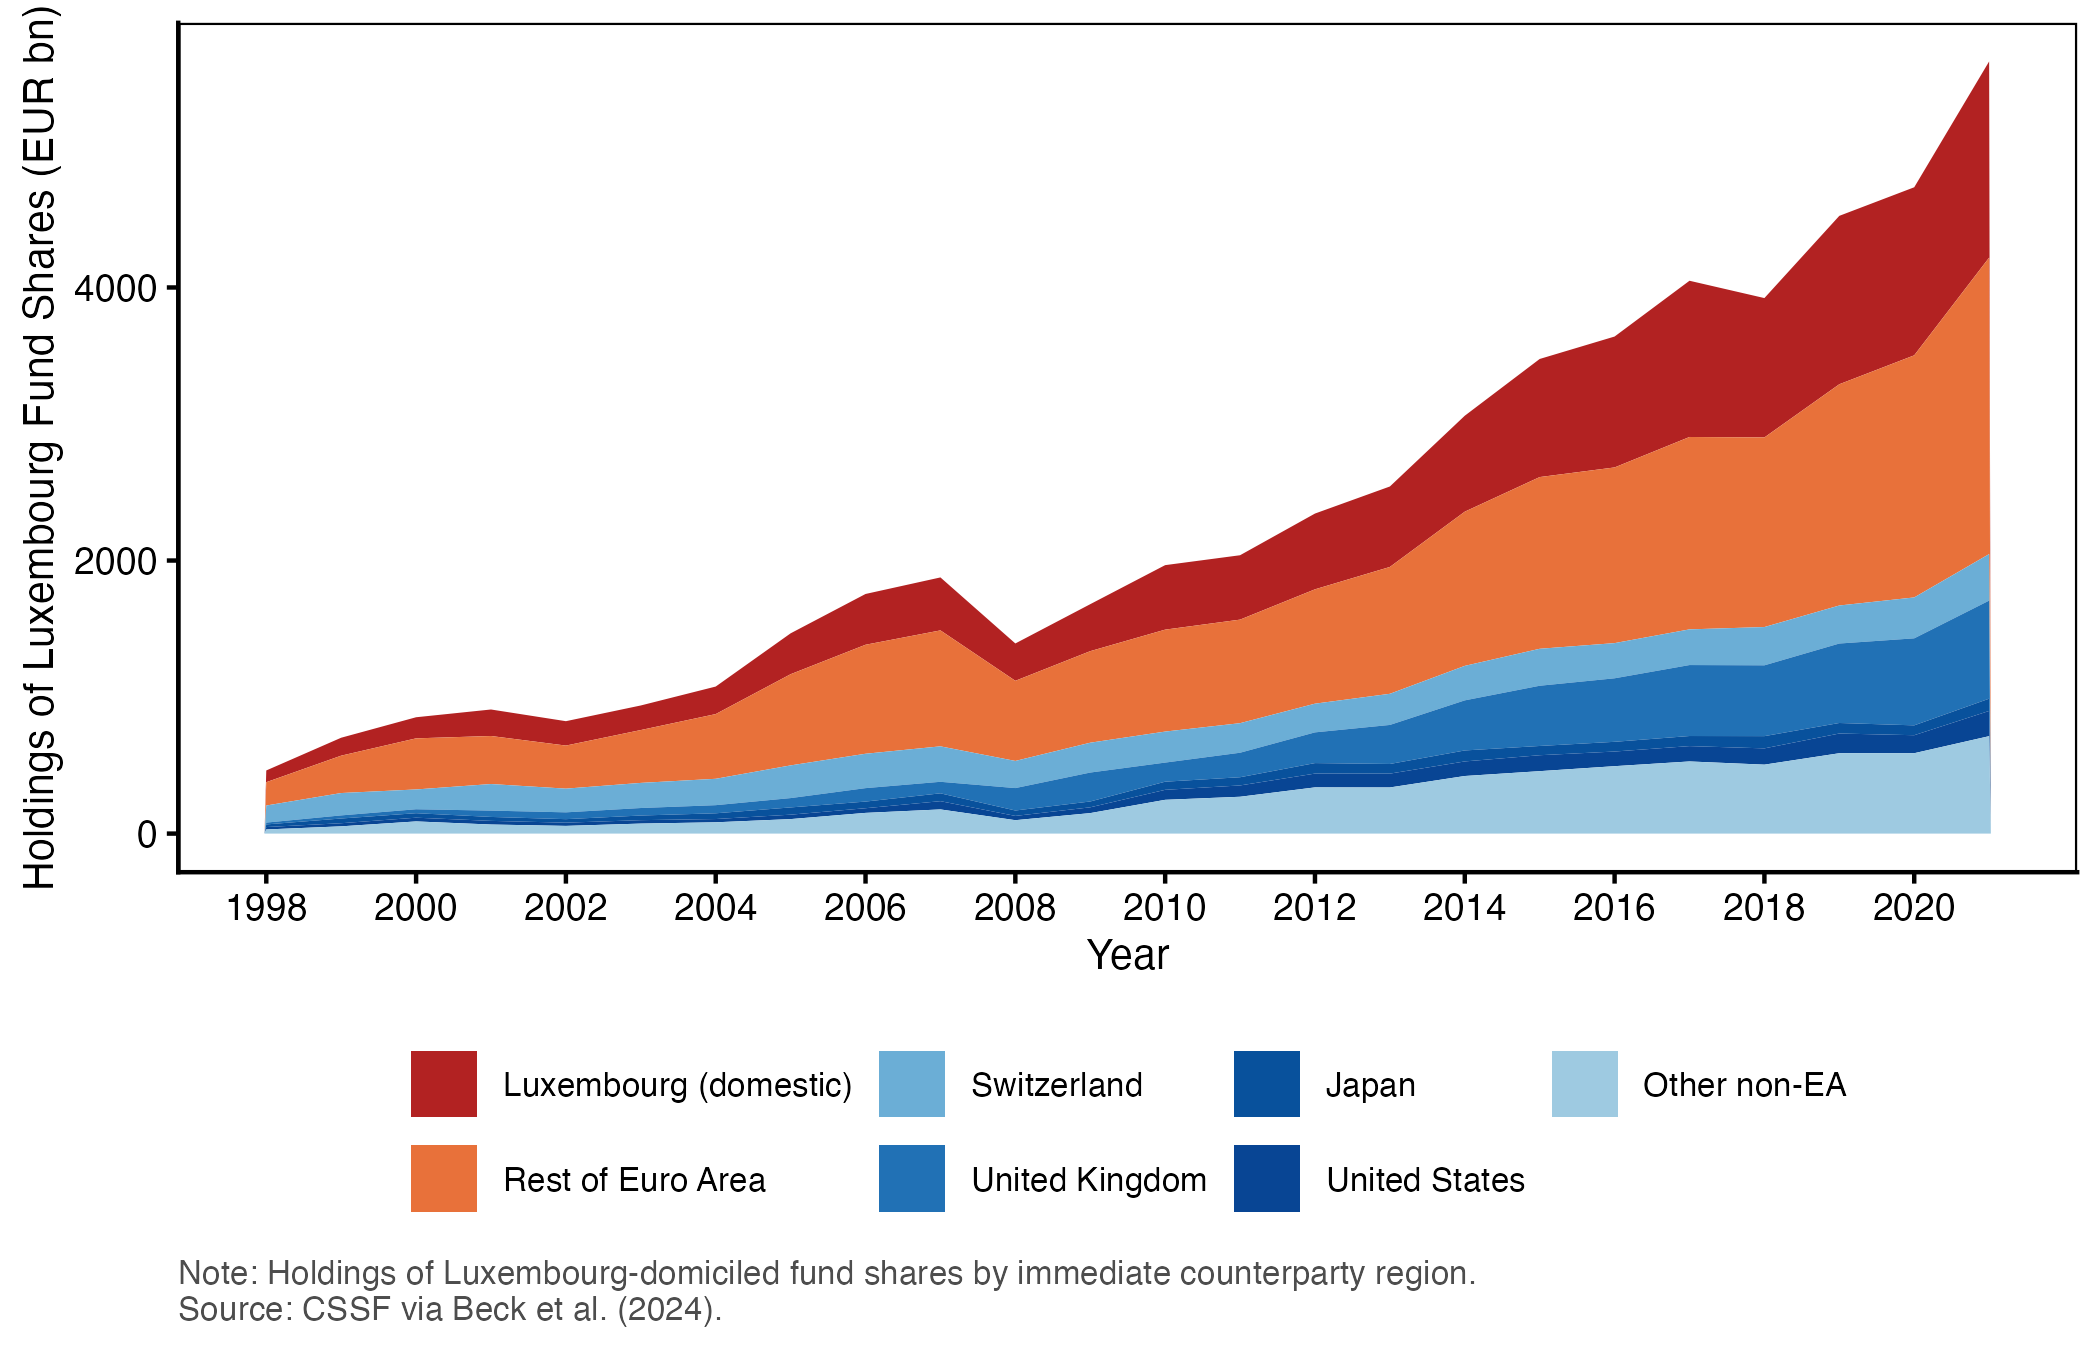
\includegraphics[width=0.9\textwidth]{../output/lux_fund_ownership_levels.png}
    \caption{Holdings of Luxembourg-domiciled fund shares in EUR billions 
    by immediate counterparty region, 1998--2021.}
    \label{fig:lux_ownership_levels}
\end{figure}

Figure~\ref{fig:irl_lux_panel} extends the analysis to Ireland using 
country-level counterparty data available for 2014--2021. The non-EA 
share is even more pronounced for Irish funds, where the United Kingdom 
alone accounts for a large fraction of total holdings. This is consistent 
with the role of Irish-domiciled funds as vehicles for UK-based 
institutional investors, including liability-driven investment (LDI) 
funds that \cite{beck2024} document in detail. The contrast between the 
two panels underscores that the misattribution problem, while present in 
both centers, operates through somewhat different investor bases.

\begin{figure}[htbp]
    \centering
    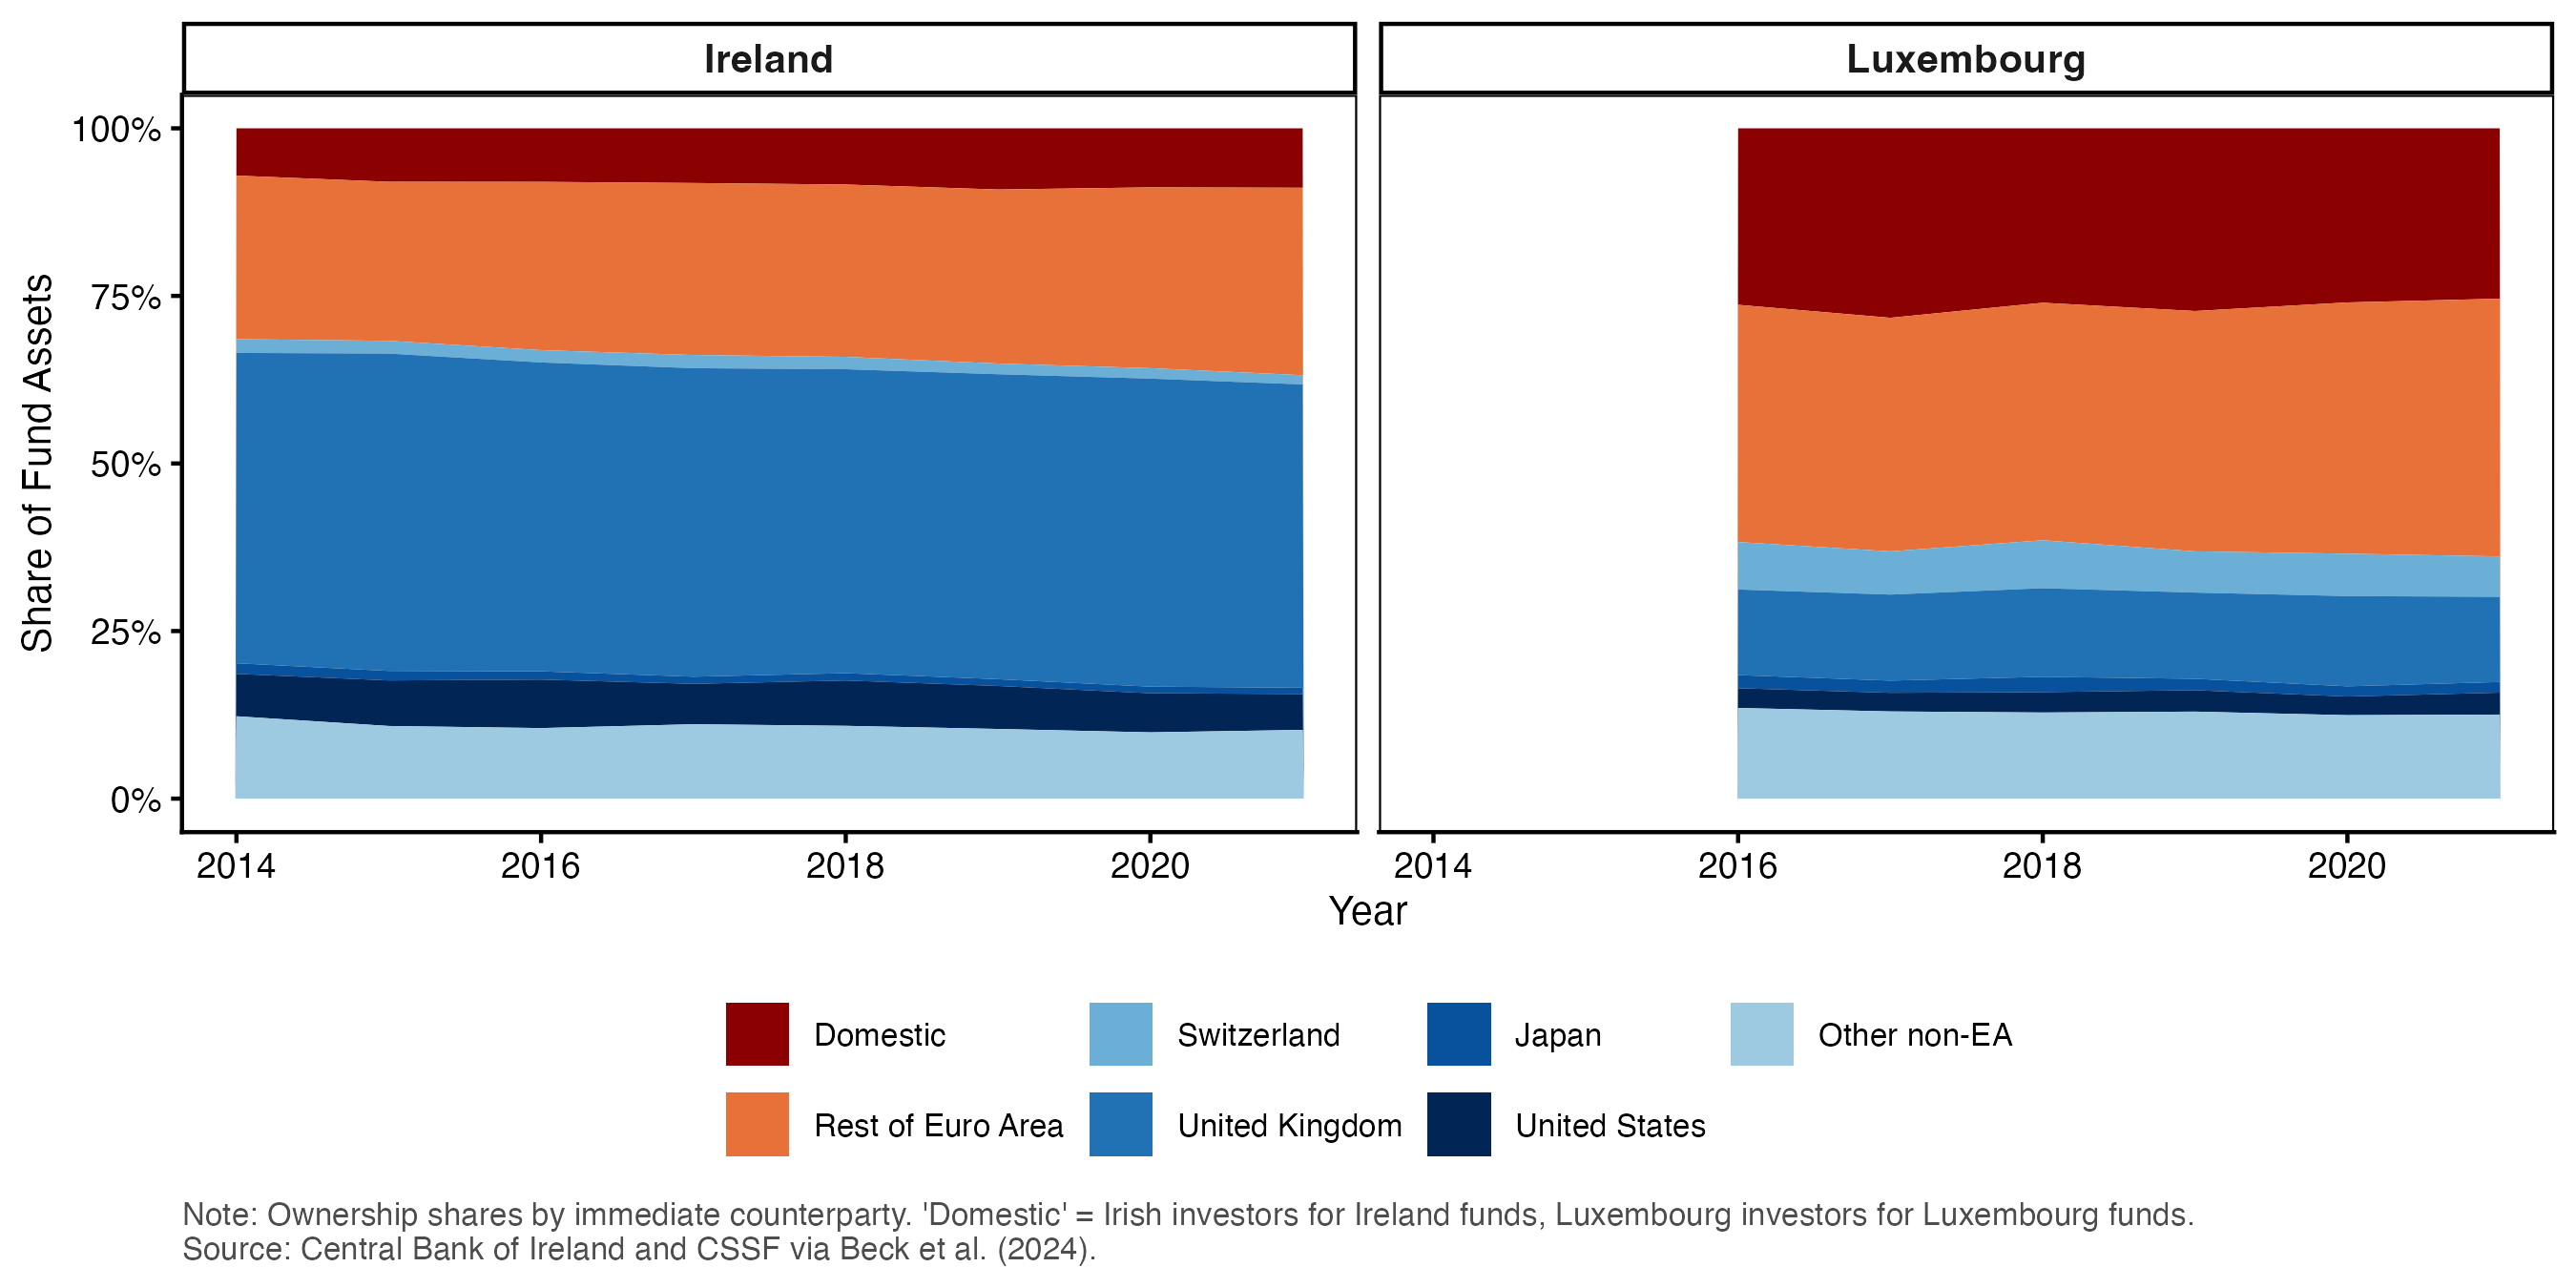
\includegraphics[width=0.95\textwidth]{../output/irl_lux_fund_ownership_shares.png}
    \caption{Ownership composition of Irish and Luxembourg fund shares by 
    immediate counterparty country, 2014--2021.}
    \label{fig:irl_lux_panel}
\end{figure}

\subsection{Geographic Reallocation of Equity Positions}

The fund counterparty statistics establish that a large share of OOFC 
fund assets belongs to non-EA investors. We now turn to the question of 
how this distorts the measured bilateral equity positions of individual 
Euro Area countries. Using the SHS-based restated bilateral portfolio 
data from \cite{beck2024}, which covers all EA countries as investors 
against approximately 240 destination countries for the period 2014--2023, 
we compare residency-based positions with fund-unwind-adjusted positions 
for selected EA economies.

Figure~\ref{fig:realloc_deu} shows Germany's top foreign equity 
destinations in 2020 under both methodologies. The contrast is stark. 
Under residency-based accounting, Luxembourg and Ireland rank among 
Germany's largest foreign equity positions, reflecting German investors' 
substantial holdings of OOFC-domiciled fund shares. After the fund 
unwind---which replaces each fund share with the underlying securities 
the fund holds---positions on Luxembourg and Ireland collapse, while 
positions on the United States and other major equity markets expand 
correspondingly. The pattern is similar for France 
(Figure~\ref{fig:realloc_fra}) and particularly pronounced for Belgium 
(Figure~\ref{fig:realloc_bel}), whose geographic proximity to Luxembourg 
is reflected in an especially large share of fund-intermediated investment.

\begin{figure}[htbp]
    \centering
    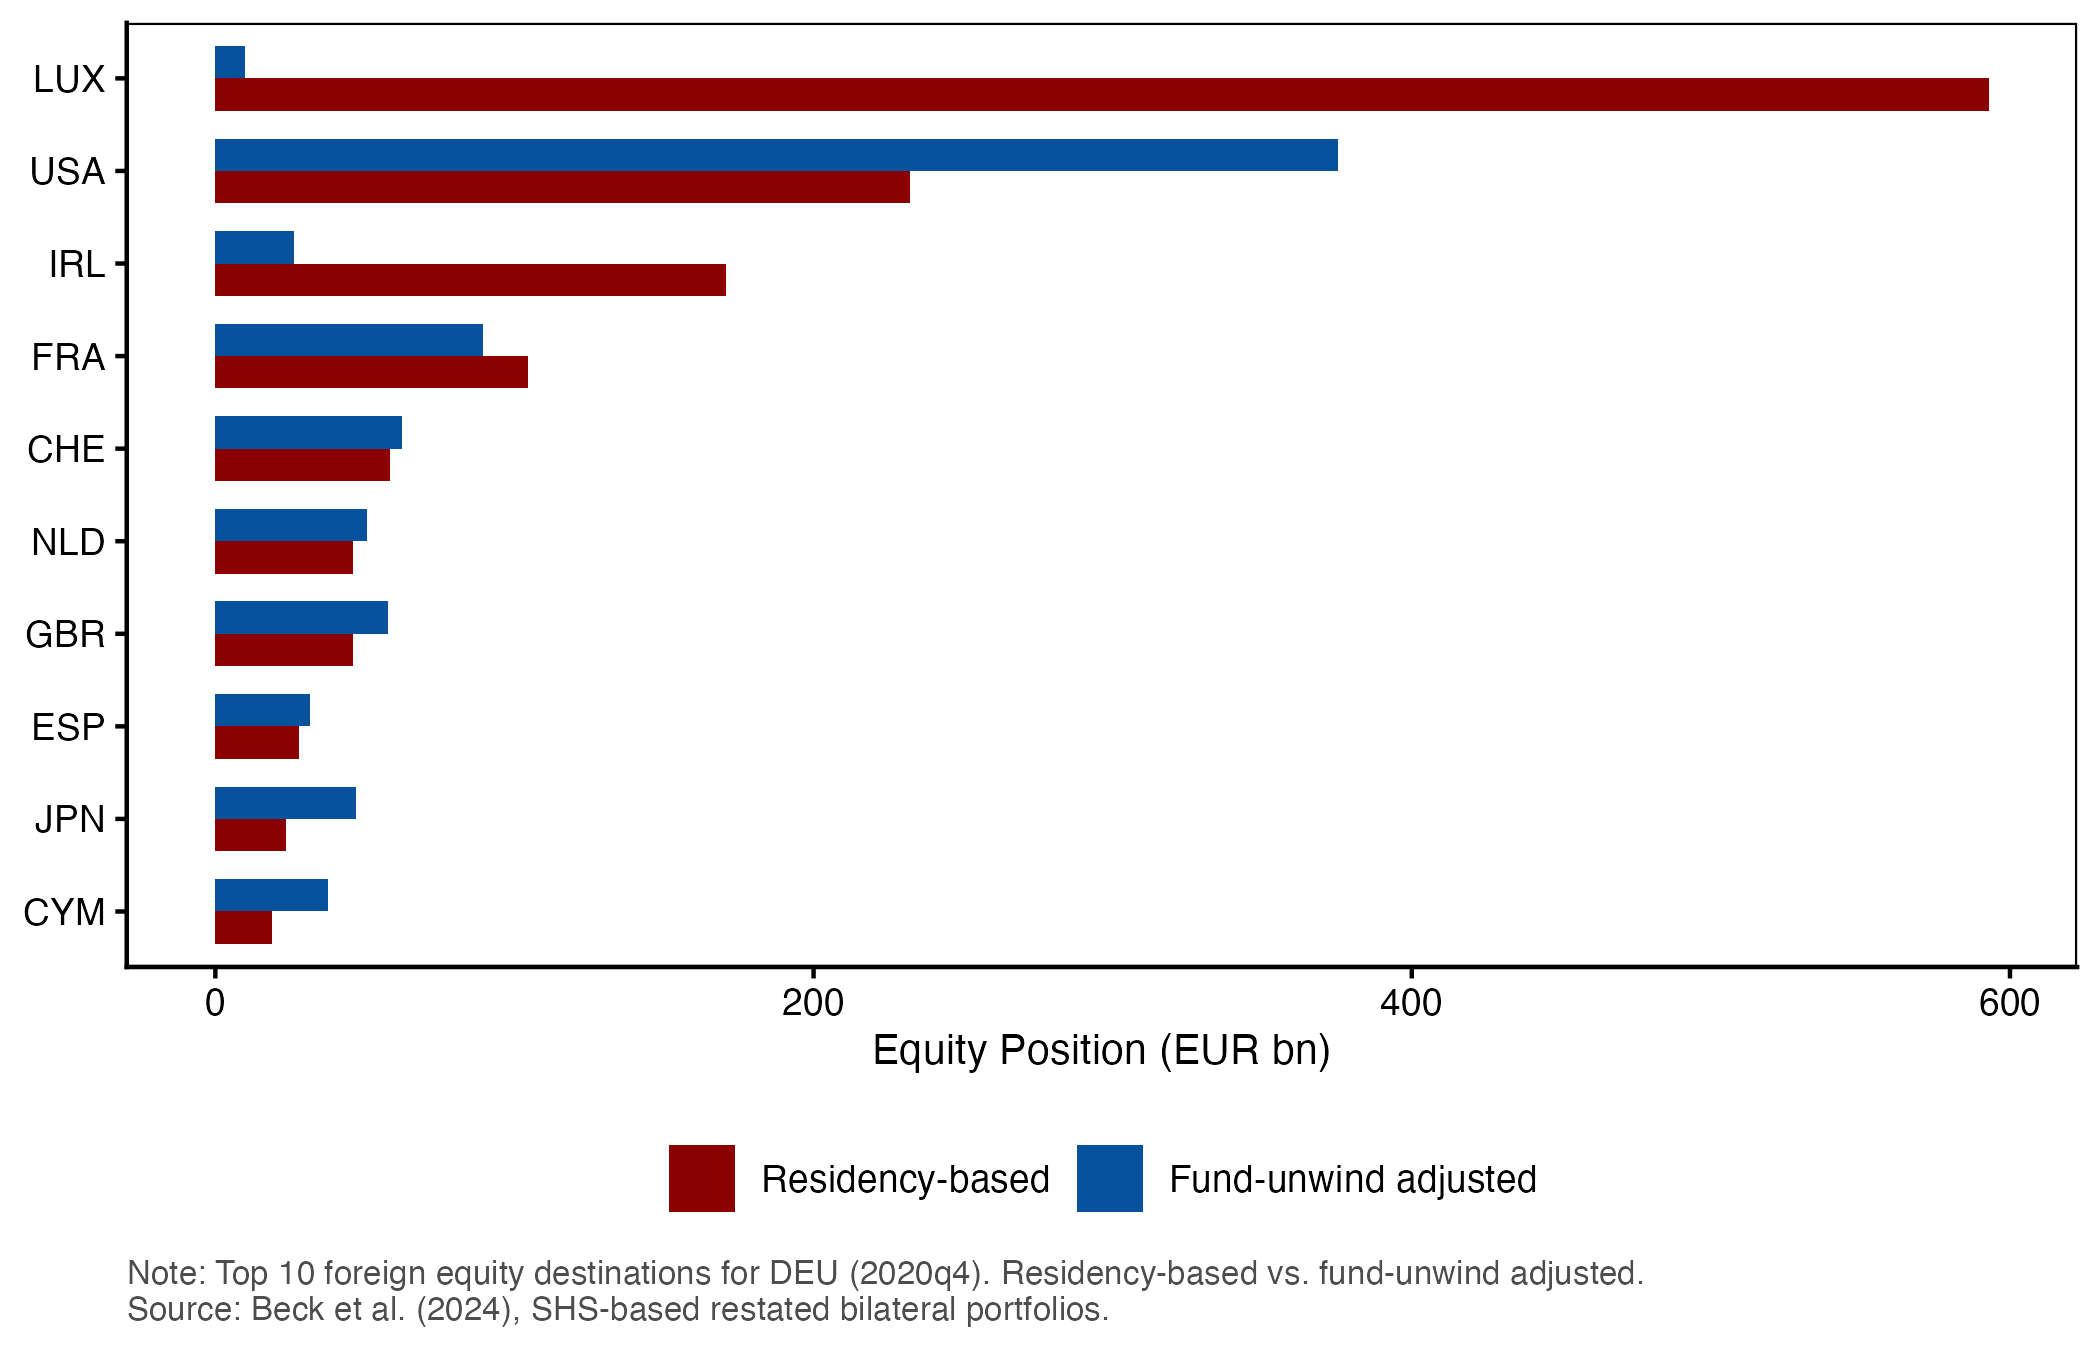
\includegraphics[width=0.85\textwidth]{../output/reallocation_deu.png}
    \caption{Germany's top foreign equity destinations: residency-based 
    vs.\ fund-unwind adjusted positions, 2020Q4.}
    \label{fig:realloc_deu}
\end{figure}

\begin{figure}[htbp]
    \centering
    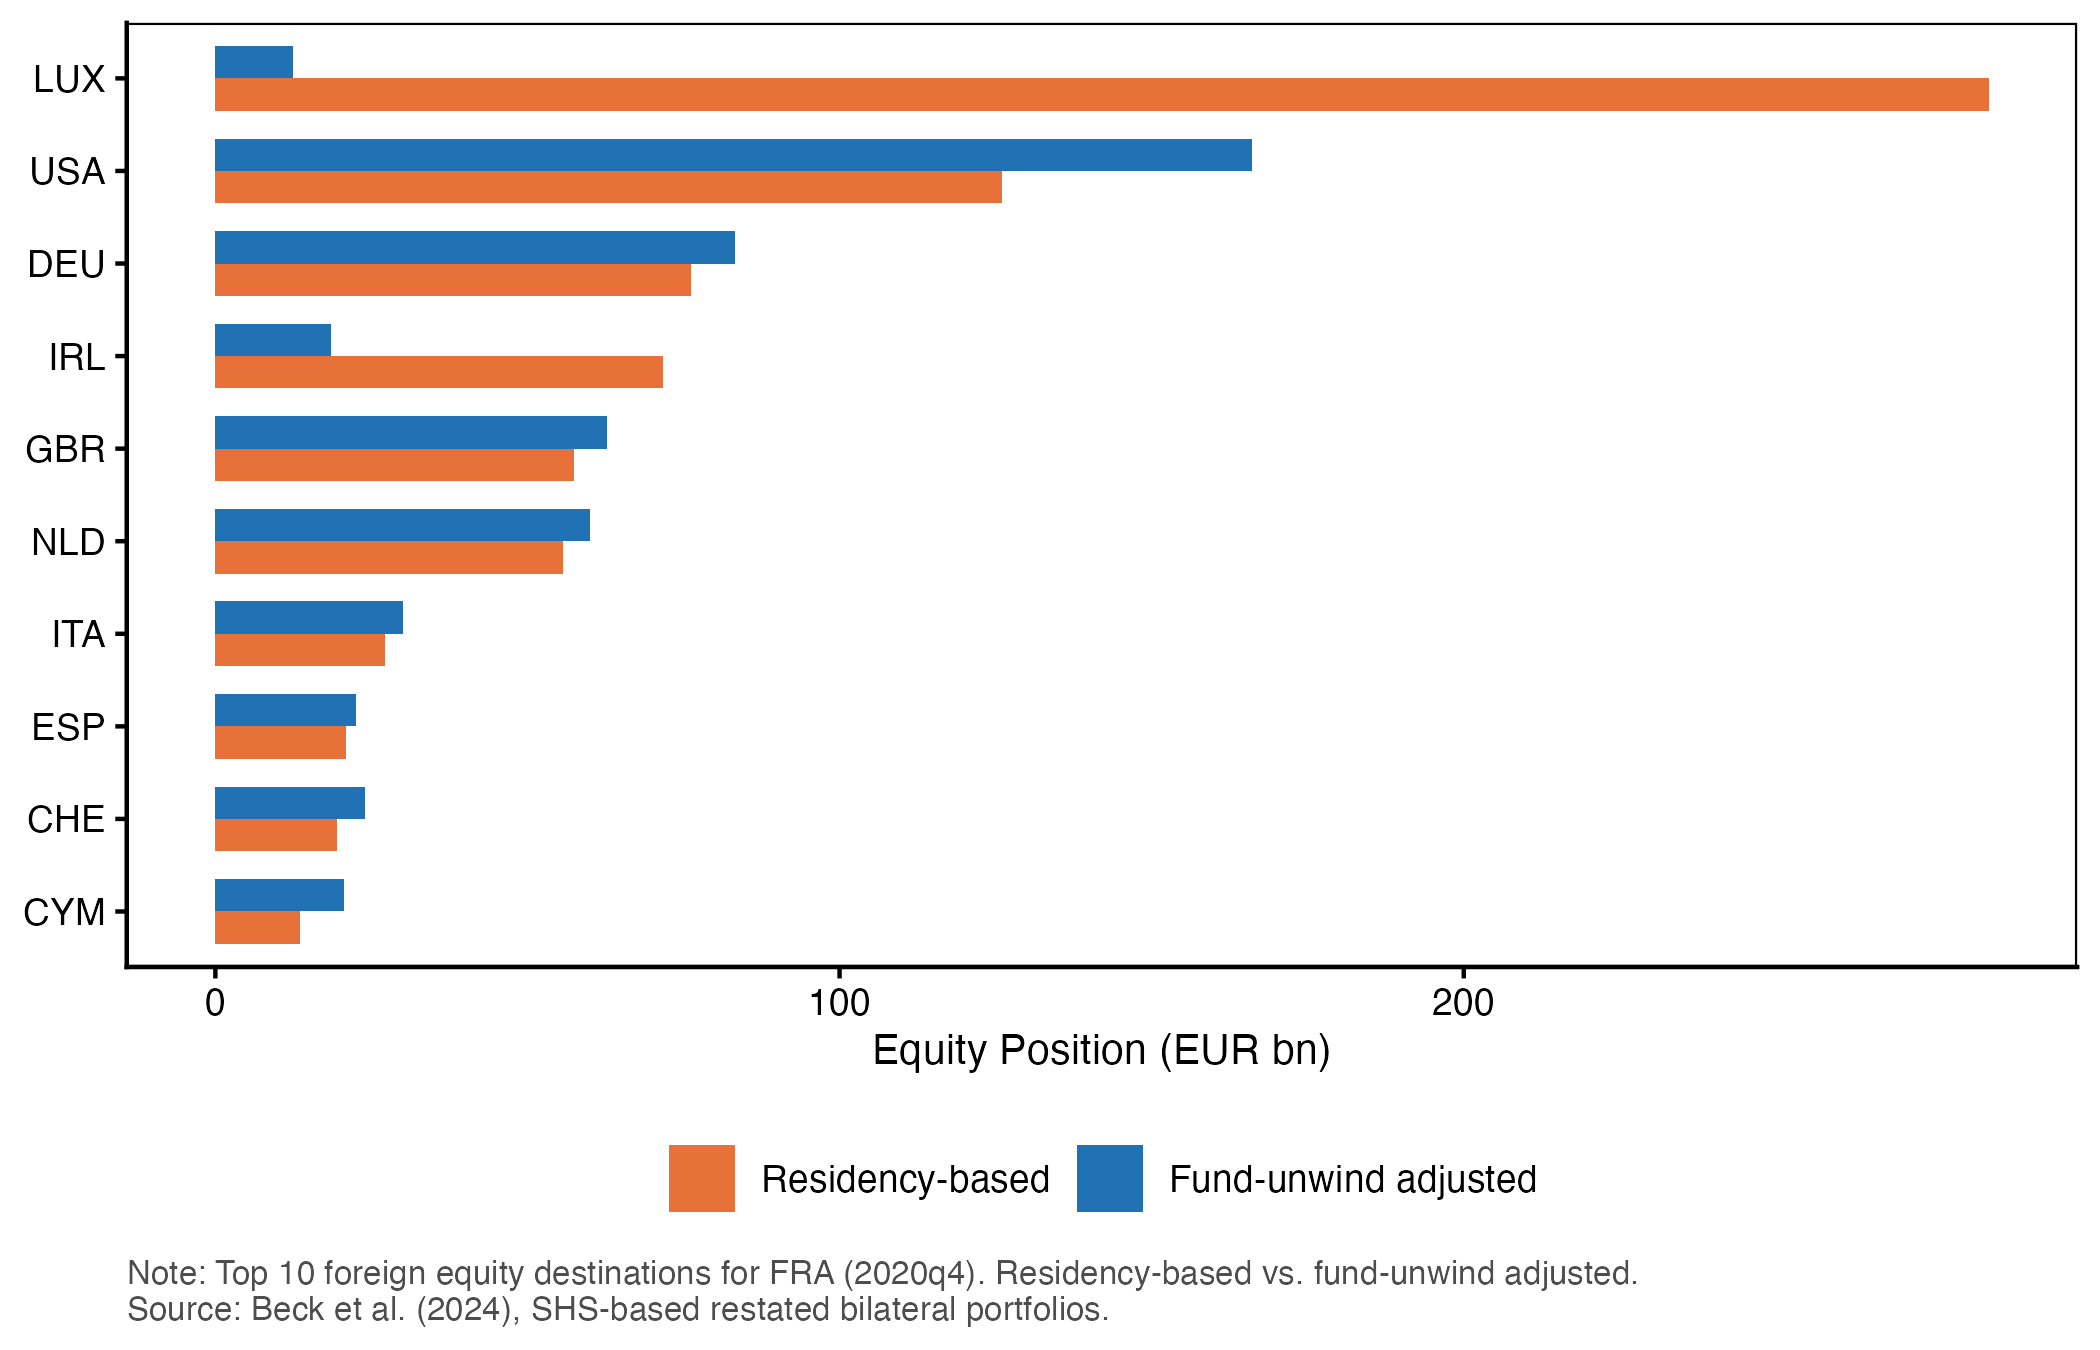
\includegraphics[width=0.85\textwidth]{../output/reallocation_fra.png}
    \caption{France's top foreign equity destinations: residency-based 
    vs.\ fund-unwind adjusted positions, 2020Q4.}
    \label{fig:realloc_fra}
\end{figure}

\begin{figure}[htbp]
    \centering
    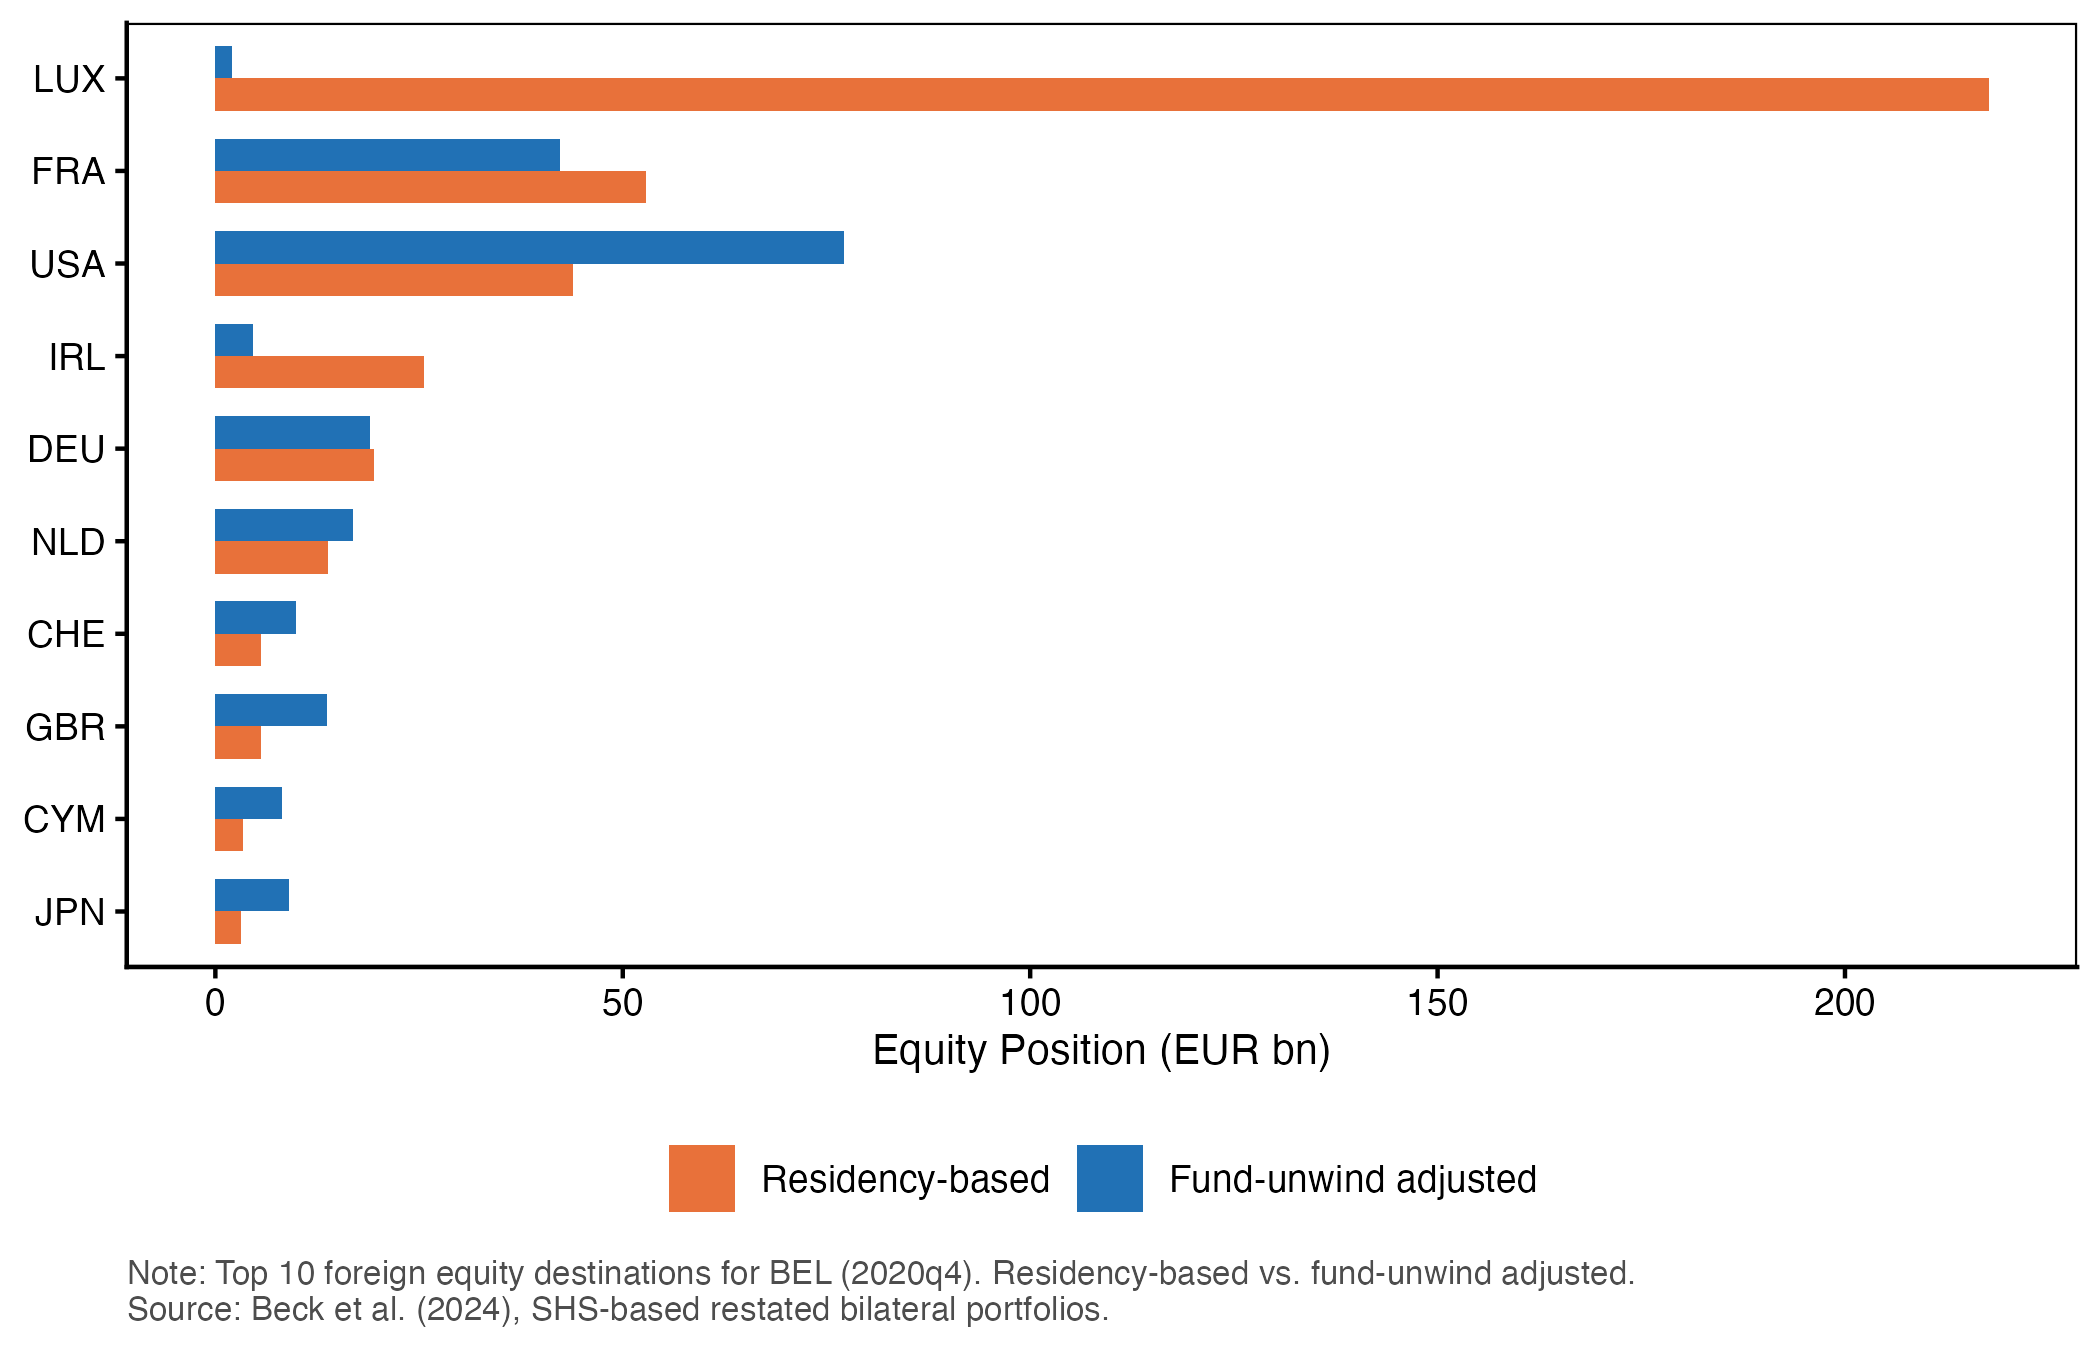
\includegraphics[width=0.85\textwidth]{../output/reallocation_bel.png}
    \caption{Belgium's top foreign equity destinations: residency-based 
    vs.\ fund-unwind adjusted positions, 2020Q4.}
    \label{fig:realloc_bel}
\end{figure}

These paired bar charts show where positions are reallocated \textit{to}, 
but do not directly reveal the extent of round-tripping---the phenomenon 
whereby an investor's holdings of OOFC fund shares partly represent 
indirect claims on domestic equities. To capture this, 
Figure~\ref{fig:net_realloc_deu} displays the net reallocation for each 
destination, defined as the difference between the fund-unwind-adjusted 
and residency-based position. Destinations with negative values (notably 
Luxembourg and Ireland) are those from which positions are reallocated 
away; destinations with positive values are those that gain exposure after 
the correction. The domestic position---labeled with the investor's own 
country code---captures the round-tripping effect: equity that appeared 
as a foreign claim on Luxembourg but is in fact an indirect holding of 
domestic securities. While the round-tripping component is non-negligible, 
it is small relative to the geographic reallocation toward the United 
States and other major markets, indicating that the primary distortion 
operates through misattribution of destination rather than through 
artificial inflation of the foreign portfolio share.

\begin{figure}[htbp]
    \centering
    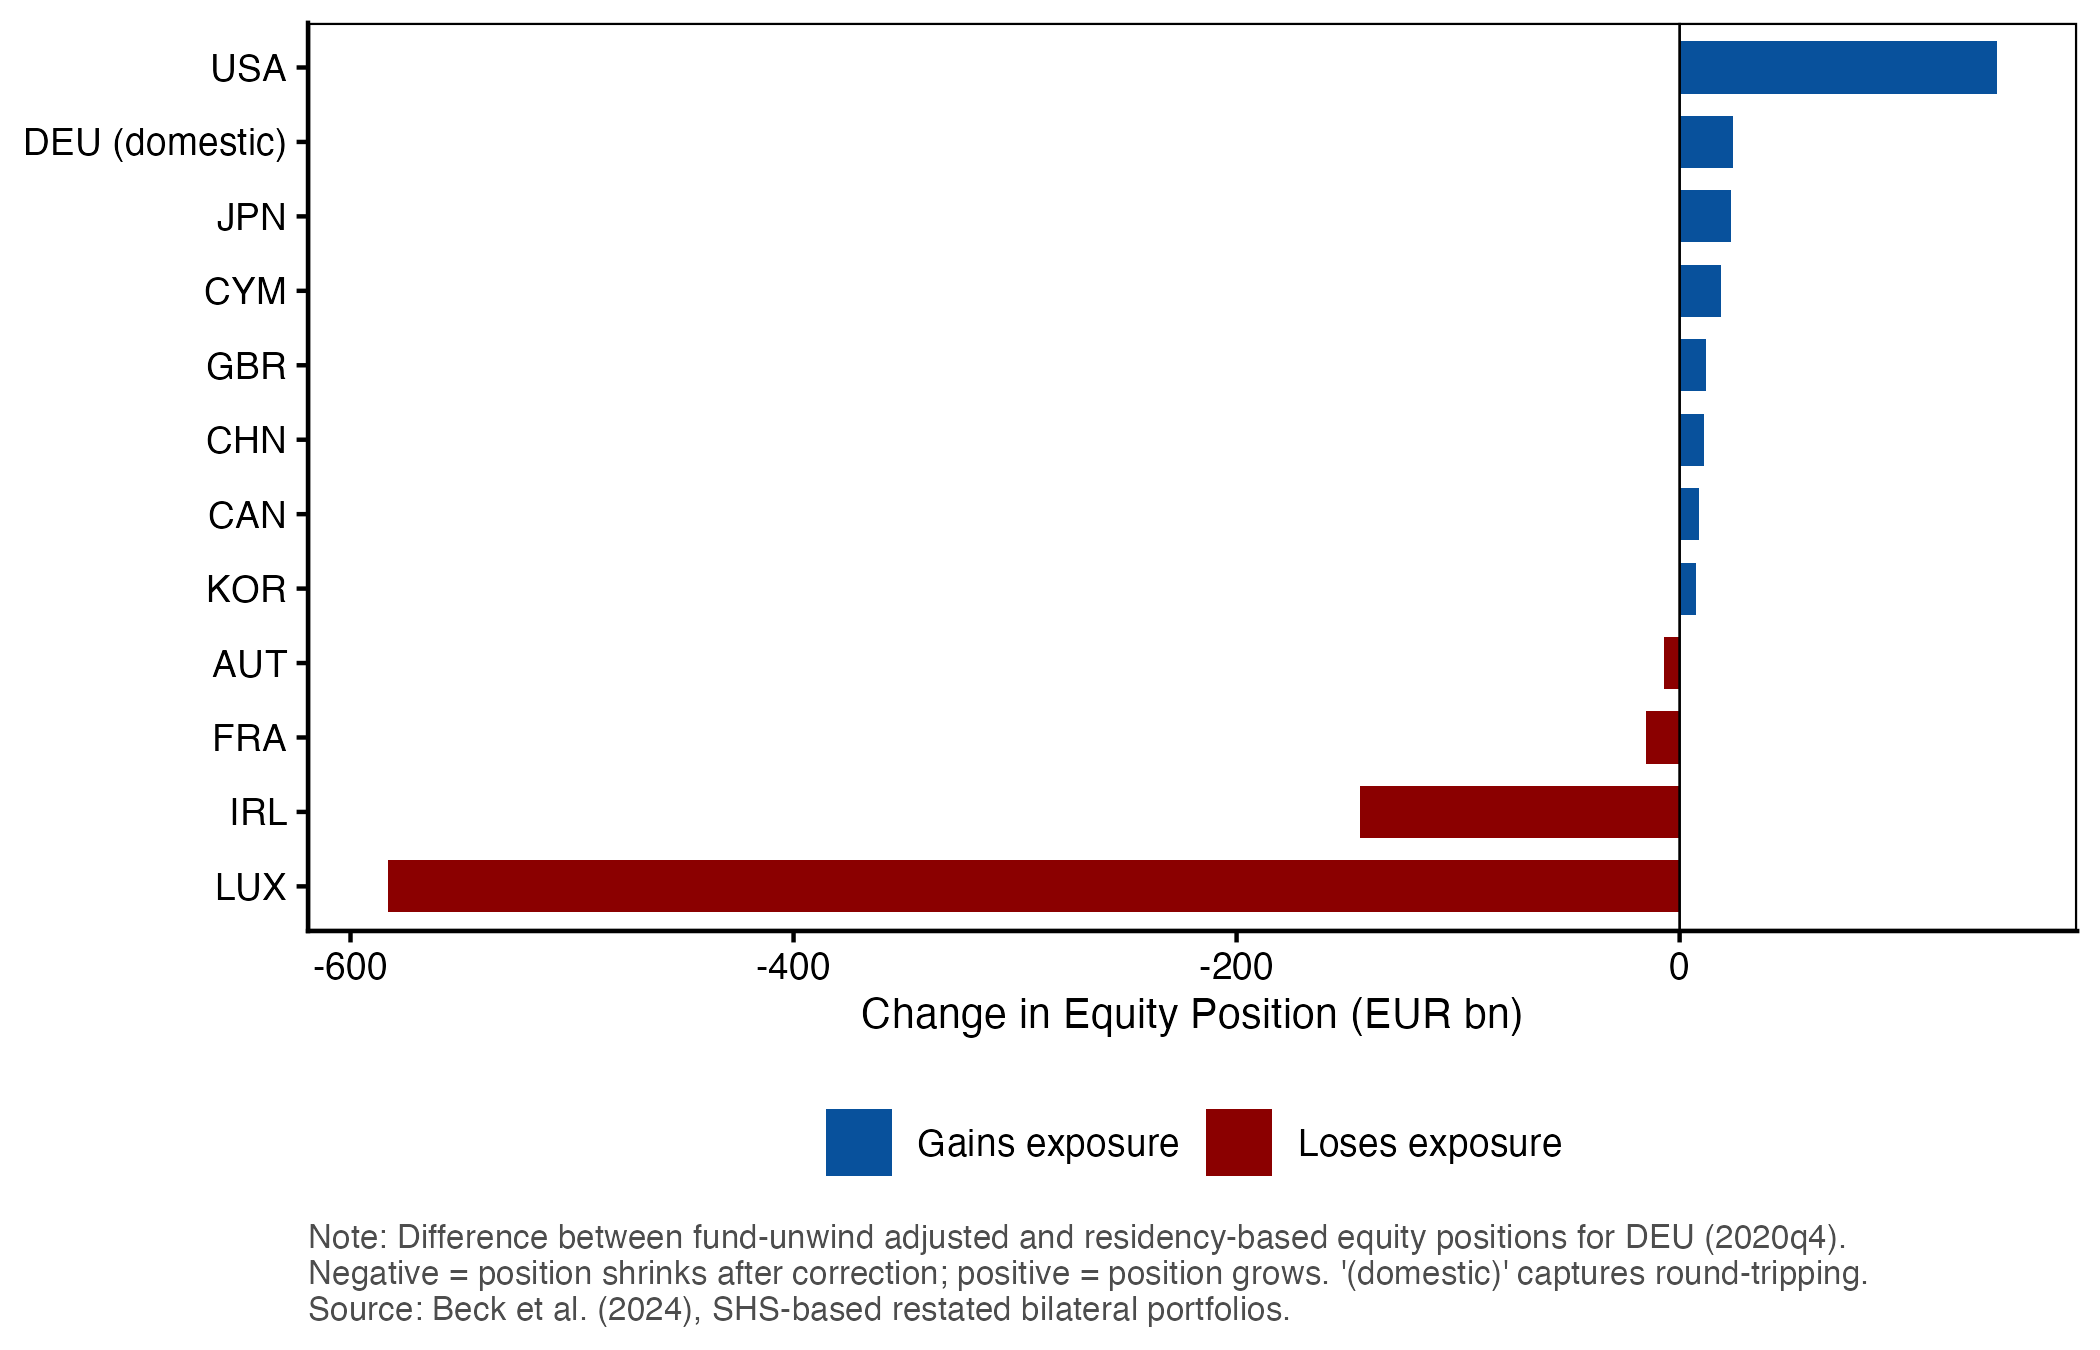
\includegraphics[width=0.85\textwidth]{../output/net_reallocation_deu.png}
    \caption{Net reallocation of Germany's equity positions after fund 
    unwind, 2020Q4. Negative values indicate positions that shrink; 
    positive values indicate positions that grow. The domestic bar 
    captures round-tripping through OOFC funds.}
    \label{fig:net_realloc_deu}
\end{figure}

\begin{figure}[htbp]
    \centering
    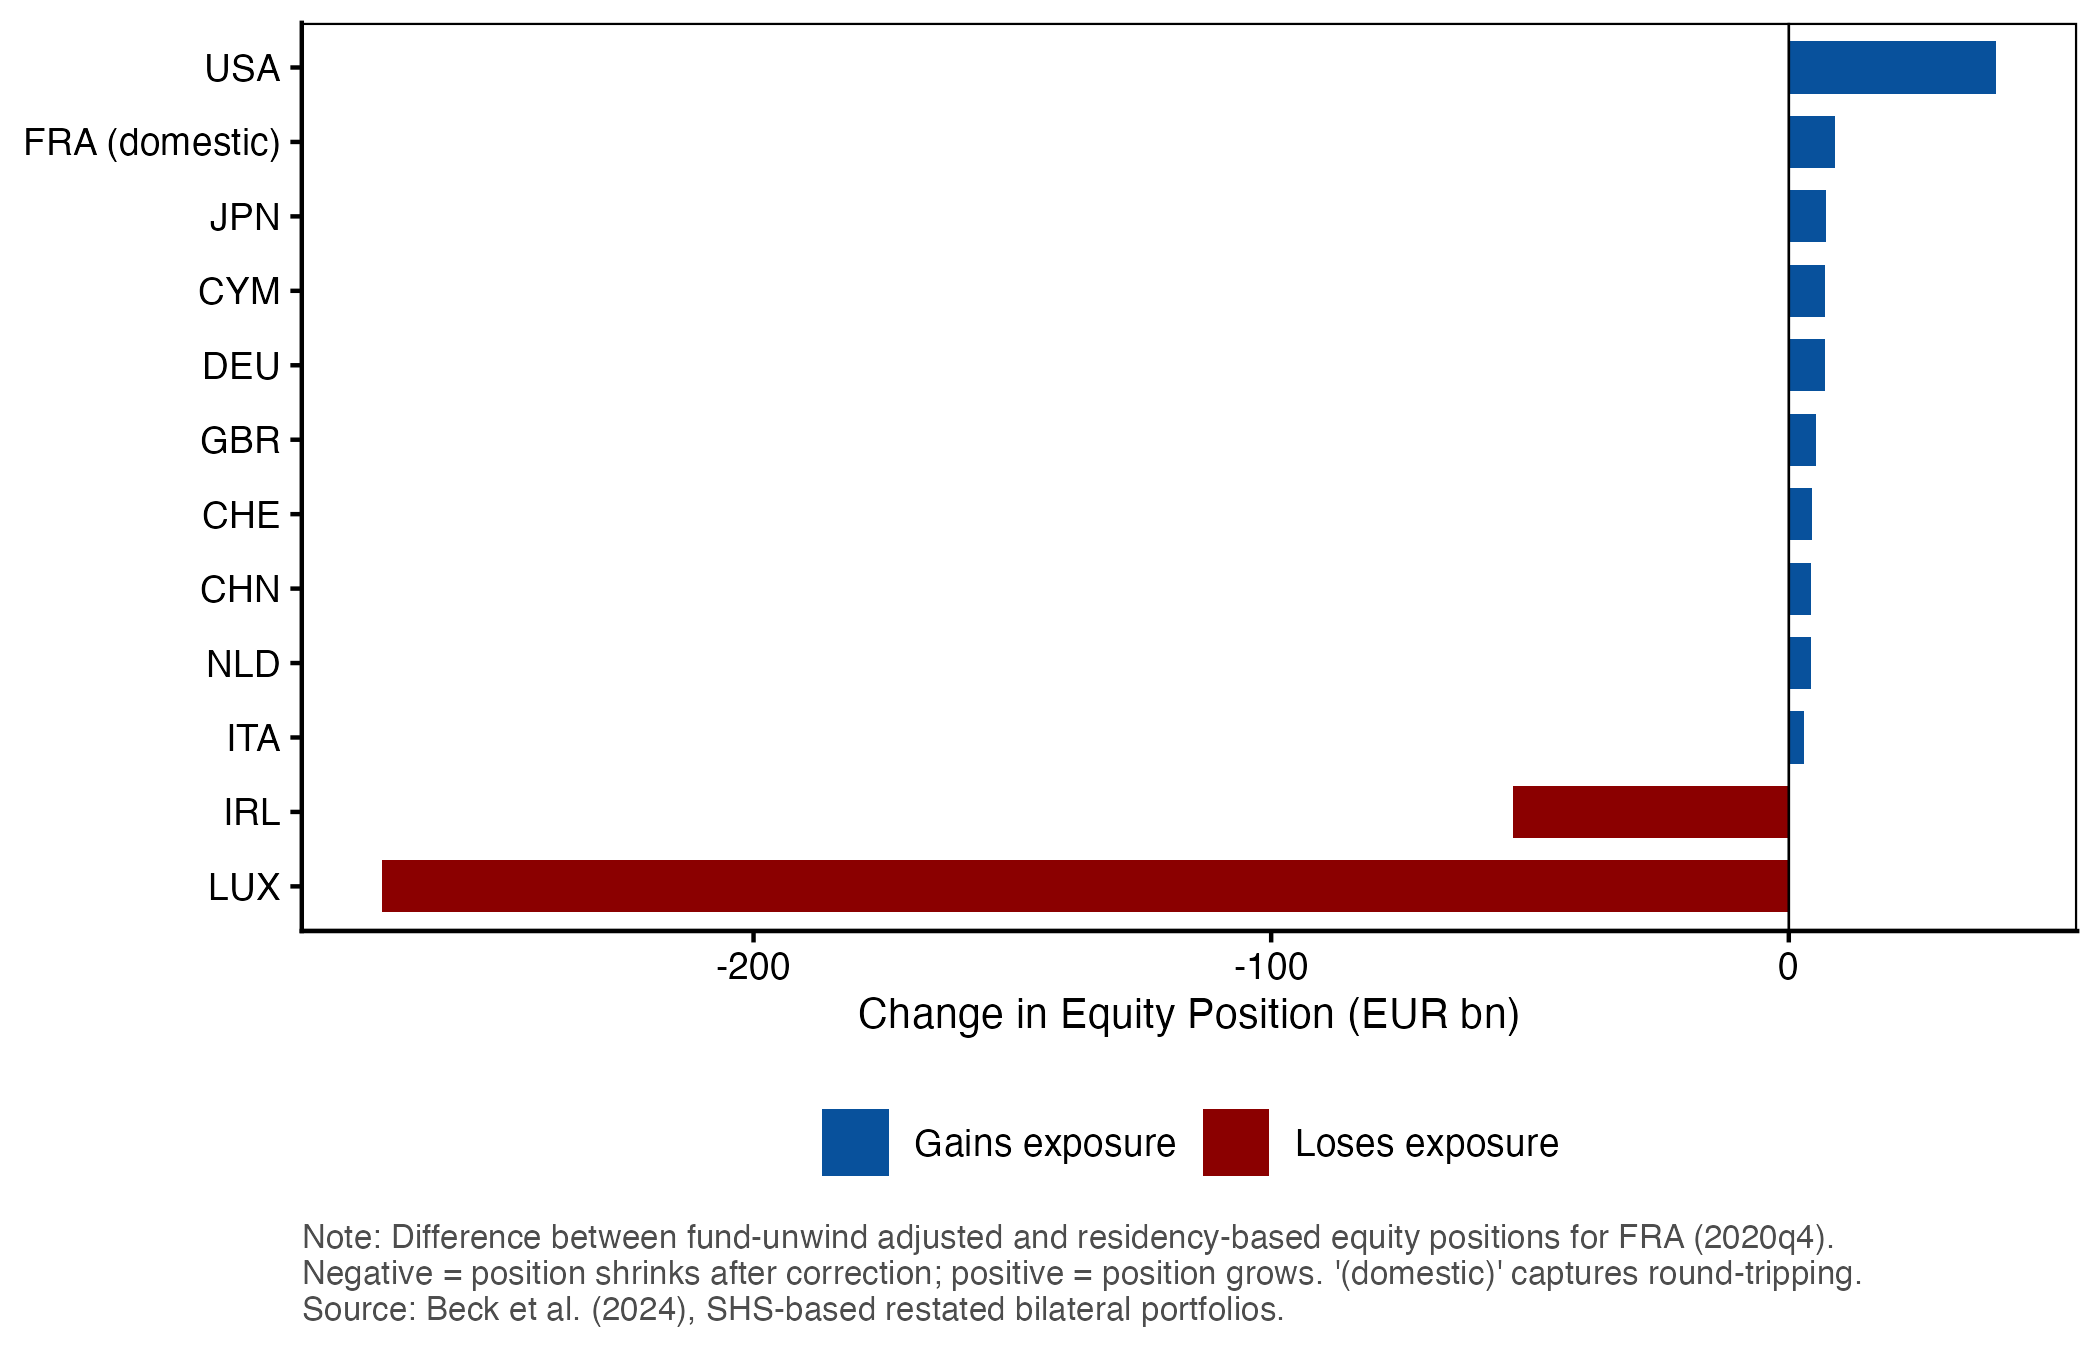
\includegraphics[width=0.85\textwidth]{../output/net_reallocation_fra.png}
    \caption{Net reallocation of France's equity positions after fund 
    unwind, 2020Q4. Negative values indicate positions that shrink; 
    positive values indicate positions that grow. The domestic bar 
    captures round-tripping through OOFC funds.}
    \label{fig:net_realloc_fra}
\end{figure}

\subsection{Implications for EWN-Based Home Bias Measures}

Having established the mechanisms through which OOFC intermediation 
distorts measured bilateral positions, we can now assess how these 
distortions affect the two EWN-based equity home bias measures presented 
in Figures~\ref{fig:ehb_groups} and~\ref{fig:ehb_ea_aggregate}: the 
average EHB across individual Euro Area countries and the EHB of the 
Euro Area treated as an aggregate.

\paragraph{Individual EA country EHB.} For the equity home bias of an 
individual country, only the \textit{total} foreign equity share matters, 
not its geographic composition. The reallocation of positions from 
Luxembourg to the United States or Japan, while substantial in bilateral 
terms, does not affect a country's measured foreign portfolio share: both 
the misattributed and the corrected positions count as foreign. The only 
channel through which the fund intermediation distortion biases individual 
countries' EHB is round-tripping---the portion of OOFC fund holdings 
that represents indirect claims on domestic equities. When a German 
investor holds a Luxembourg fund that in turn holds German equities, 
this position is recorded as a foreign claim on Luxembourg rather than 
a domestic holding. Foreign equity assets are therefore overstated, 
domestic holdings understated, and the resulting EHB is biased downward. 
As Figure~\ref{fig:net_realloc_deu} illustrates, this round-tripping 
component exists but is modest relative to the total portfolio. The 
downward bias in individual EA countries' EHB from the EWN data is 
therefore present but limited in magnitude, and our finding that EA 
countries experienced a stronger EHB decline than non-EA OECD countries 
is unlikely to be entirely driven by this distortion---though it may 
be somewhat exaggerated.
The country average we used excluded Ireland and Luxembourg whichs EHB is very distorted.

\paragraph{Euro Area aggregate EHB.} The distortion operates through an 
entirely different channel at the aggregate level. When the Euro Area is 
treated as a single entity, intra-EA cross-border holdings are 
reclassified as domestic. This consolidation eliminates both the 
round-tripping problem (indirect domestic claims via OOFC funds are 
domestic from the aggregate perspective regardless) and the intra-EA 
geographic misattribution (a German claim recorded against Luxembourg 
but actually representing French equity is intra-EA in all cases). 
The distortion that \textit{does not} cancel at the aggregate level is 
the presence of rest-of-world investors in OOFC-domiciled funds. When a 
US or UK investor holds shares in a Luxembourg fund that invests in 
non-EA equities, the fund's assets are recorded as Luxembourg's---and 
therefore the Euro Area's---foreign equity claims on the rest of the 
world. In reality, this represents rest-of-world capital investing in 
rest-of-world equities, with Luxembourg serving merely as an 
intermediary. This channel inflates the Euro Area aggregate's measured 
foreign equity position and biases its EHB downward. As the fund 
counterparty statistics in Figure~\ref{fig:lux_ownership} demonstrate, 
non-EA investors account for more than half of Luxembourg fund assets 
throughout the sample period, and the absolute magnitude of this 
misattribution has grown from hundreds of billions to several trillion 
euros---explaining why the Euro Area aggregate EHB declined so 
dramatically in the EWN data despite the consolidation of intra-EA 
positions.

This asymmetry between debt and equity integration carries implications 
beyond the measurement debate. In the framework of \cite{sorensen2007}, 
it is equity diversification---not debt---that drives income risk sharing 
through cross-border ownership of productive assets. The finding that 
the euro successfully integrated bond markets but left equity home bias 
at levels comparable to non-EA economies suggests that the currency 
union has delivered integration in precisely the asset class where the 
risk-sharing gains are smallest, while the channel that matters most 
for consumption smoothing remains underdeveloped. This resonates with 
ongoing policy discussions around the European Capital Markets Union 
and the diagnosis in the \cite{draghi2024} report, which identifies 
the fragmentation of European equity and venture capital markets as a 
key barrier to innovation and growth. The persistent equity home bias 
within the Euro Area---even after two decades of monetary 
integration---underscores that a common currency alone is insufficient 
to overcome the structural, regulatory, and informational barriers to 
cross-border equity investment, and that deeper capital market 
integration may require the kind of institutional reforms currently 
under discussion, including elements of a banking union and harmonized 
insolvency and securities regulation.